% !TEX root = ../thesis.tex

% Appendices: invoked after \appendix in thesis.tex.

\chapter{Hyperparameter Tables}
\label{app:hyperparameters}

% TODO: One \section per generator with a tabular layout listing every
% hyperparameter actually used in the runs that produced the synthetic
% files in thesis/data/<generator>/. Pull values from the source files:
%   - HealthGAN:    ../../healthgan/generators/wgan_for_mac.py (params dict)
%   - PATE-GAN:     ../../Pategan/generate_pategan_synthetic.py (CLI defaults)
%   - Pythia-70M:   ../../pythia/generate_pythia_synthetic.py --model pythia-70m
%   - Pythia-1B:    ../../pythia/generate_pythia_synthetic.py --model pythia-1b
%   - Pythia-1B-DP: ../../pythia/generate_pythia_synthetic_dp.py (CLI
%                   defaults + DPConfig)

\section{HealthGAN (WGAN-GP)}
% TODO: table — base_nodes, critic_iters, lambda, num_epochs, batch_size,
% Adam (lr, beta1, beta2), random_state.

\section{PATE-GAN}
% TODO: table — k (teachers), n_s, batch_size, lambda (Laplace), epsilon,
% delta, RMSprop lr, weight clip range.

\section{Pythia-70M (LoRA)}
% TODO: table — base model = EleutherAI/pythia-70m, LoRA r/alpha/dropout,
% epochs, batch_size, lr, max_length, temperature, top_p,
% max_retries_per_row, generation_batch_size, seed.

\section{Pythia-1B (LoRA)}
% TODO: table — base model = EleutherAI/pythia-1b, identical LoRA and
% generation configuration to Pythia-70M; record only the deltas.

\section{Pythia-1B-DP (LoRA + Opacus)}
% TODO: table — same as Pythia-1B plus target_epsilon, target_delta,
% max_grad_norm, per_device_batch_size, gradient_accumulation_steps,
% effective_batch_size, achieved_epsilon (from run_metadata_dp.json).

% --------------------------------------------------------------

\chapter{Per-Column Distribution Plots}
\label{app:distributions}

This appendix provides the complete per-column marginal gallery summarised
in Section~\ref{sec:results:rq2:utility:similarity}, where only the first
two column blocks are reproduced in the main text
(Figure~\ref{fig:rq2:marginals}). Each figure overlays the real reference
and all five synthetic generators for a block of columns; the column range
is annotated in each panel title. Across every block the same pattern
holds: HealthGAN and the three Pythia variants track the real marginals,
whereas PATE-GAN distorts both categorical and continuous columns.

\begin{figure}[H]
\centering
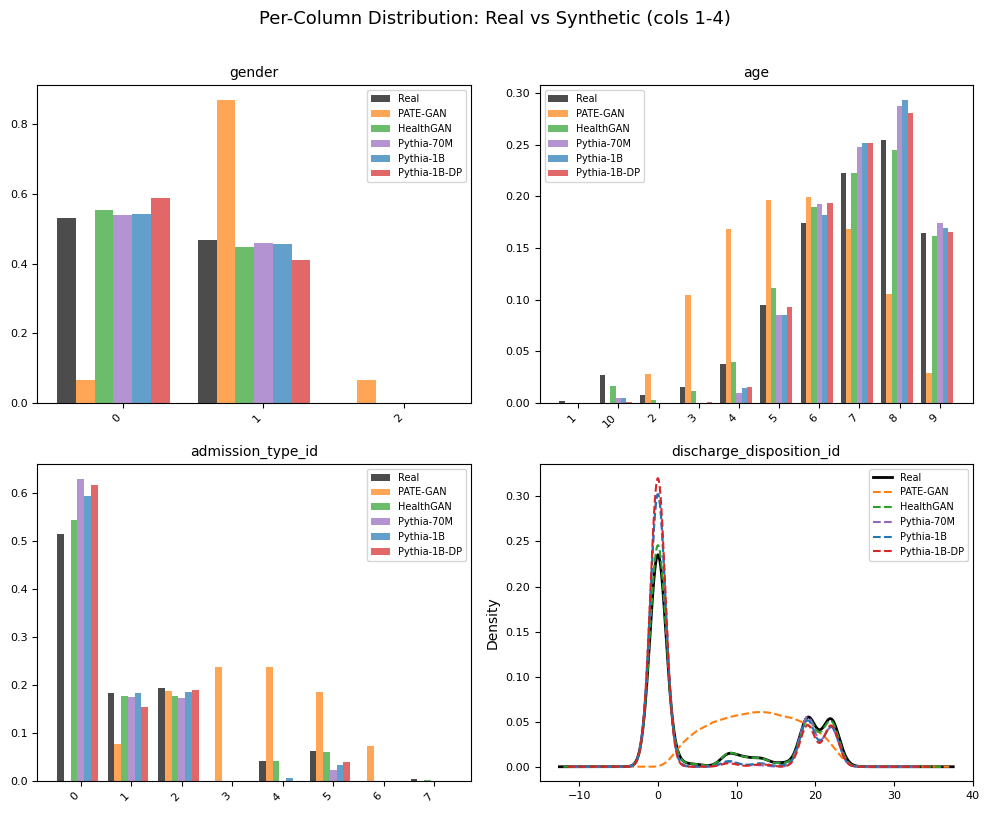
\includegraphics[width=0.95\textwidth]{images/results/marginals_0}
\caption{Per-column marginal distributions, real versus all five
generators (block 1 of 5).}
\label{app:fig:marg0}
\end{figure}

\begin{figure}[H]
\centering
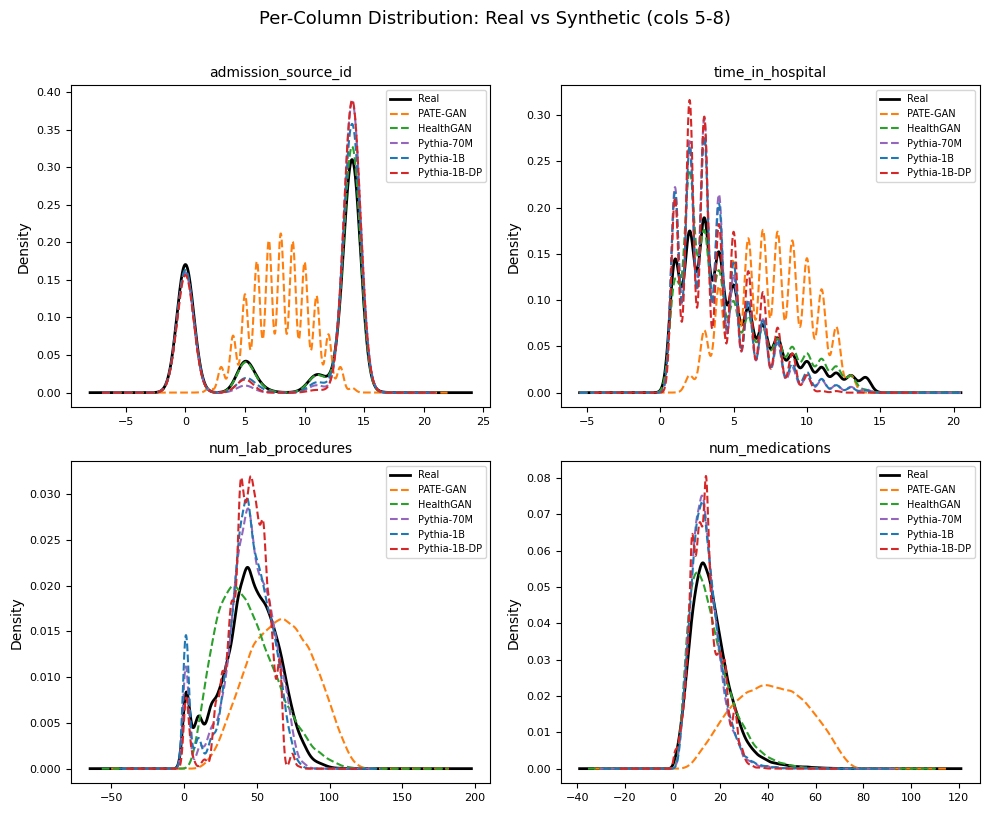
\includegraphics[width=0.95\textwidth]{images/results/marginals_1}
\caption{Per-column marginal distributions, real versus all five
generators (block 2 of 5).}
\label{app:fig:marg1}
\end{figure}

\begin{figure}[H]
\centering
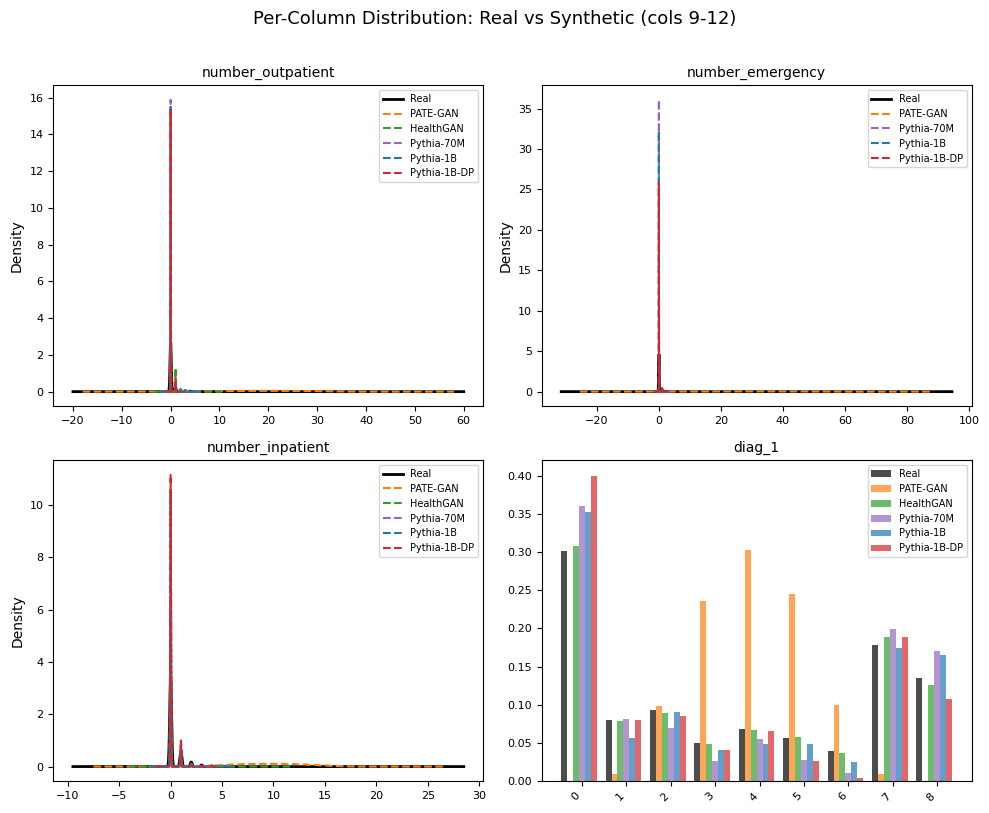
\includegraphics[width=0.95\textwidth]{images/results/marginals_2}
\caption{Per-column marginal distributions, real versus all five
generators (block 3 of 5).}
\label{app:fig:marg2}
\end{figure}

\begin{figure}[H]
\centering
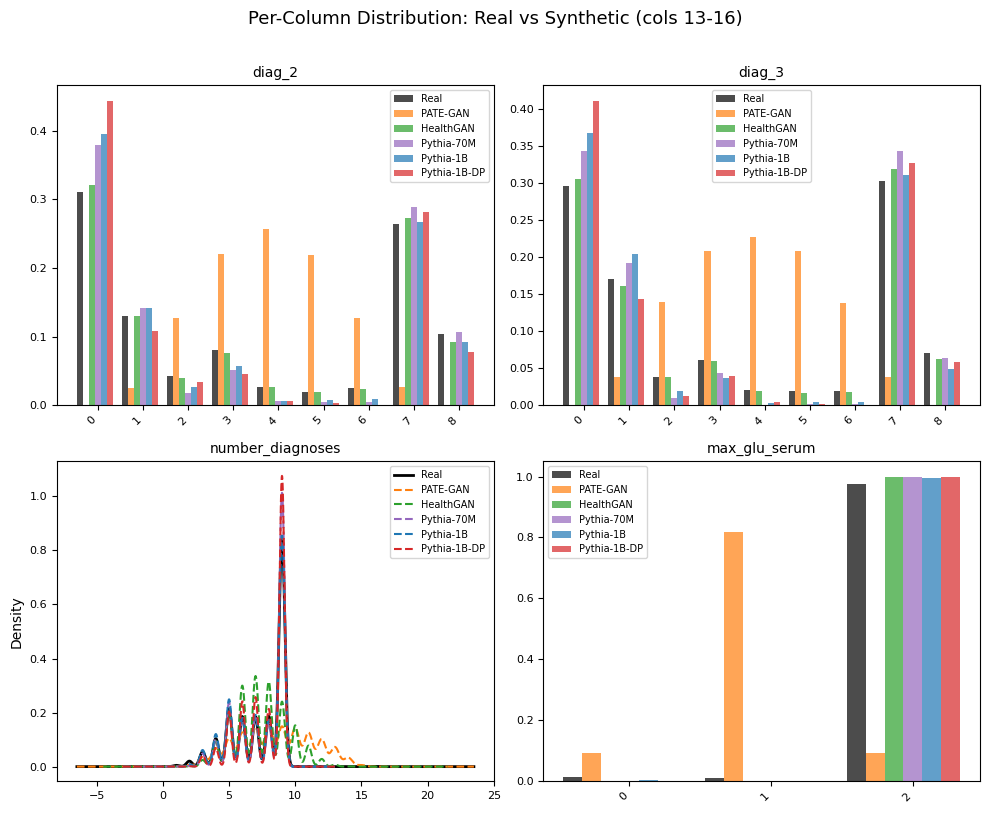
\includegraphics[width=0.95\textwidth]{images/results/marginals_3}
\caption{Per-column marginal distributions, real versus all five
generators (block 4 of 5).}
\label{app:fig:marg3}
\end{figure}

\begin{figure}[H]
\centering
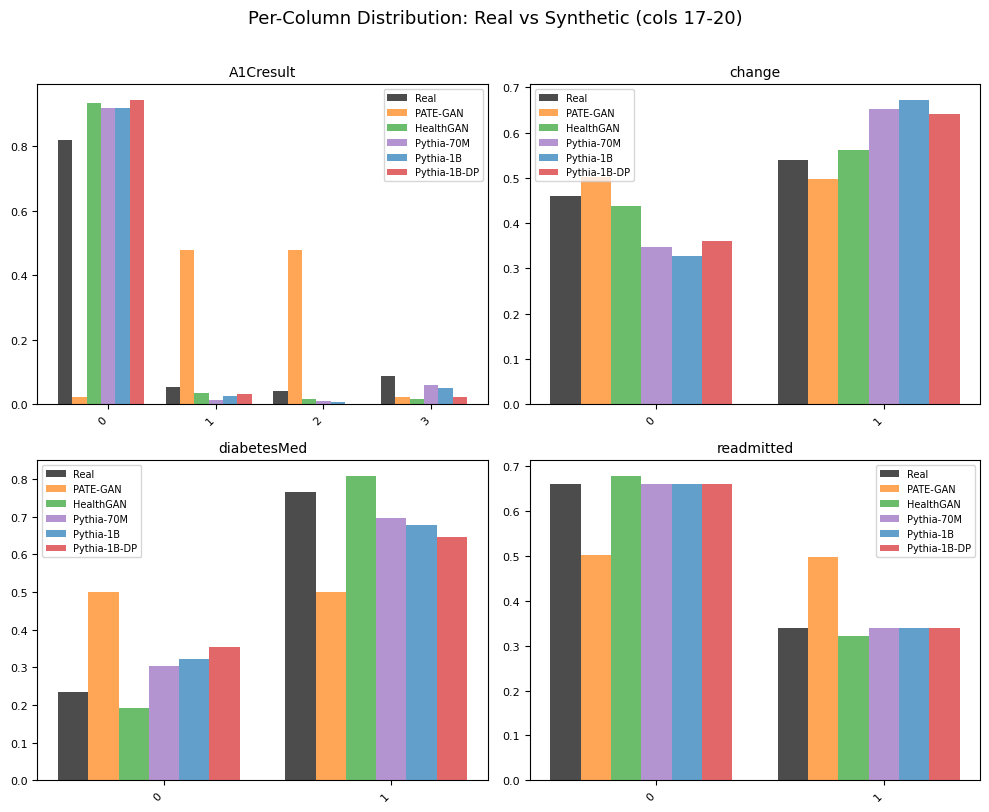
\includegraphics[width=0.95\textwidth]{images/results/marginals_4}
\caption{Per-column marginal distributions, real versus all five
generators (block 5 of 5).}
\label{app:fig:marg4}
\end{figure}

% --------------------------------------------------------------

\chapter{Per-Generator Utility Diagnostics}
\label{app:utility-diag}

The main text reports the class-balance, train--test, correlation-difference,
and survival diagnostics of Section~\ref{sec:results:rq2:utility} in
compressed form. This appendix provides the supporting tables and the full
per-generator visual diagnostics.

\section{Class-Balance and Train--Test Diagnostics}
\label{app:class-balance}

Figure~\ref{app:fig:class-balance} and Table~\ref{app:tab:class-balance}
show the positive-class prevalence of the binary readmission target in the
real and synthetic train/test splits. Table~\ref{app:tab:train-test-auc}
then reports the full AUC-ROC matrix for the TRTR, TSTR, TRTS, and TSTS
regimes.

\begin{figure}[H]
\centering
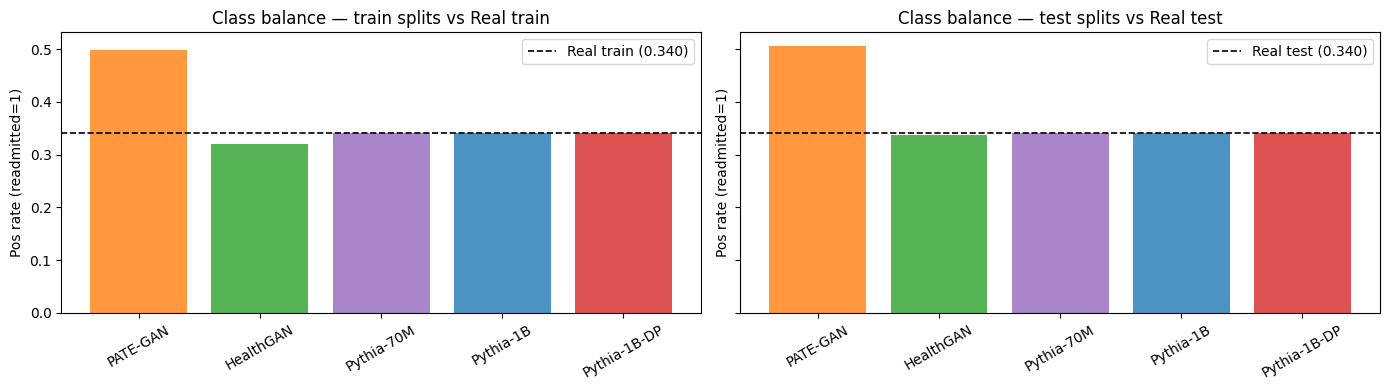
\includegraphics[width=\textwidth]{images/results/class_balance}
\caption{Class balance of the binary readmission target in real and
synthetic train/test splits. The dashed line marks the corresponding
real-split prevalence.}
\label{app:fig:class-balance}
\end{figure}

\begin{table}[H]
\centering
\small
\caption{Readmission class balance by source and split. $\Delta$ is computed
against the matching real split.}
\label{app:tab:class-balance}
\begin{tabular}{llrrrrr}
\toprule
Source & Split & $N$ & Pos (1) & Neg (0) & Pos rate & $\Delta$ vs Real \\
\midrule
Real        & train & 57{,}214 & 19{,}464 & 37{,}750 & 0.340 & $+0.000$ \\
Real        & test  & 14{,}304 & 4{,}866  & 9{,}438  & 0.340 & $+0.000$ \\
PATE-GAN    & train & 57{,}214 & 28{,}500 & 28{,}714 & 0.498 & $+0.158$ \\
HealthGAN   & train & 57{,}214 & 18{,}345 & 38{,}869 & 0.321 & $-0.020$ \\
Pythia-70M  & train & 57{,}214 & 19{,}464 & 37{,}750 & 0.340 & $+0.000$ \\
Pythia-1B   & train & 57{,}214 & 19{,}464 & 37{,}750 & 0.340 & $+0.000$ \\
Pythia-1B-DP & train & 57{,}214 & 19{,}464 & 37{,}750 & 0.340 & $+0.000$ \\
PATE-GAN    & test  & 14{,}304 & 7{,}245  & 7{,}059  & 0.507 & $+0.166$ \\
HealthGAN   & test  & 14{,}304 & 4{,}813  & 9{,}491  & 0.336 & $-0.004$ \\
Pythia-70M  & test  & 14{,}304 & 4{,}866  & 9{,}438  & 0.340 & $+0.000$ \\
Pythia-1B   & test  & 14{,}304 & 4{,}866  & 9{,}438  & 0.340 & $+0.000$ \\
Pythia-1B-DP & test  & 14{,}304 & 4{,}866  & 9{,}438  & 0.340 & $+0.000$ \\
\bottomrule
\end{tabular}
\end{table}

\begin{table}[H]
\centering
\scriptsize
\caption{AUC-ROC by train--test regime. TSTR is the headline downstream
utility regime; TRTS checks synthetic test realism, and TSTS checks internal
synthetic consistency.}
\label{app:tab:train-test-auc}
\begin{tabular}{llcccc}
\toprule
Synthetic Source & Classifier & TRTR & TSTR & TRTS & TSTS \\
\midrule
HealthGAN & Gradient Boosting & 0.7008 & 0.6312 & 0.6531 & 0.6191 \\
HealthGAN & Logistic Regression & 0.6670 & 0.6130 & 0.6499 & 0.6103 \\
HealthGAN & Random Forest & 0.6790 & 0.6153 & 0.6366 & 0.6021 \\
\midrule
PATE-GAN & Gradient Boosting & 0.7008 & 0.5108 & 0.4601 & 0.5323 \\
PATE-GAN & Logistic Regression & 0.6670 & 0.5079 & 0.5082 & 0.5432 \\
PATE-GAN & Random Forest & 0.6790 & 0.5018 & 0.5040 & 0.5302 \\
\midrule
Pythia-1B & Gradient Boosting & 0.7008 & 0.6818 & 0.6980 & 0.7119 \\
Pythia-1B & Logistic Regression & 0.6670 & 0.6613 & 0.6822 & 0.6969 \\
Pythia-1B & Random Forest & 0.6790 & 0.6682 & 0.6635 & 0.8343 \\
\midrule
Pythia-1B-DP & Gradient Boosting & 0.7008 & 0.5827 & 0.5338 & 0.5403 \\
Pythia-1B-DP & Logistic Regression & 0.6670 & 0.5868 & 0.5013 & 0.5236 \\
Pythia-1B-DP & Random Forest & 0.6790 & 0.5823 & 0.5353 & 0.6213 \\
\midrule
Pythia-70M & Gradient Boosting & 0.7008 & 0.6634 & 0.5939 & 0.5920 \\
Pythia-70M & Logistic Regression & 0.6670 & 0.6573 & 0.5882 & 0.5893 \\
Pythia-70M & Random Forest & 0.6790 & 0.6588 & 0.5678 & 0.5720 \\
\bottomrule
\end{tabular}
\end{table}

\section{Correlation-Difference Heatmaps}
\label{app:corrheat}

Figure~\ref{app:fig:corrheat} gives the correlation-difference heatmaps
(real minus synthetic correlation matrix) for all five generators,
extending the contrast of Figure~\ref{fig:rq2:corrheat}. Saturated cells
denote large residual correlation; pale cells denote faithful
reproduction of the pairwise dependency structure.

\begin{figure}[H]
\centering
\begin{subfigure}{0.48\textwidth}\centering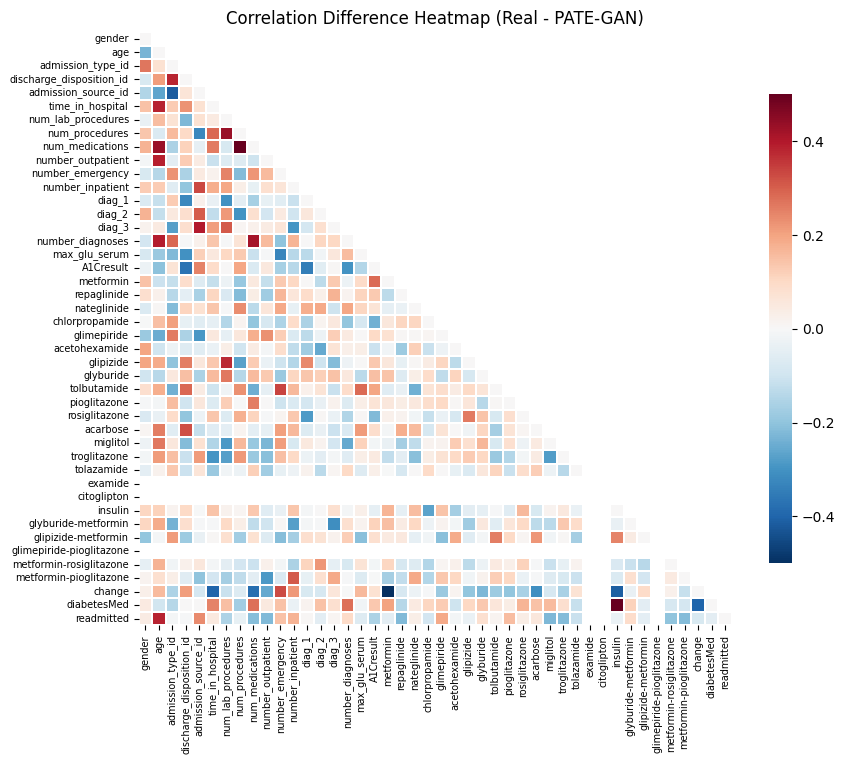
\includegraphics[width=\textwidth]{images/results/corrheat_0}\caption{PATE-GAN}\end{subfigure}\hfill
\begin{subfigure}{0.48\textwidth}\centering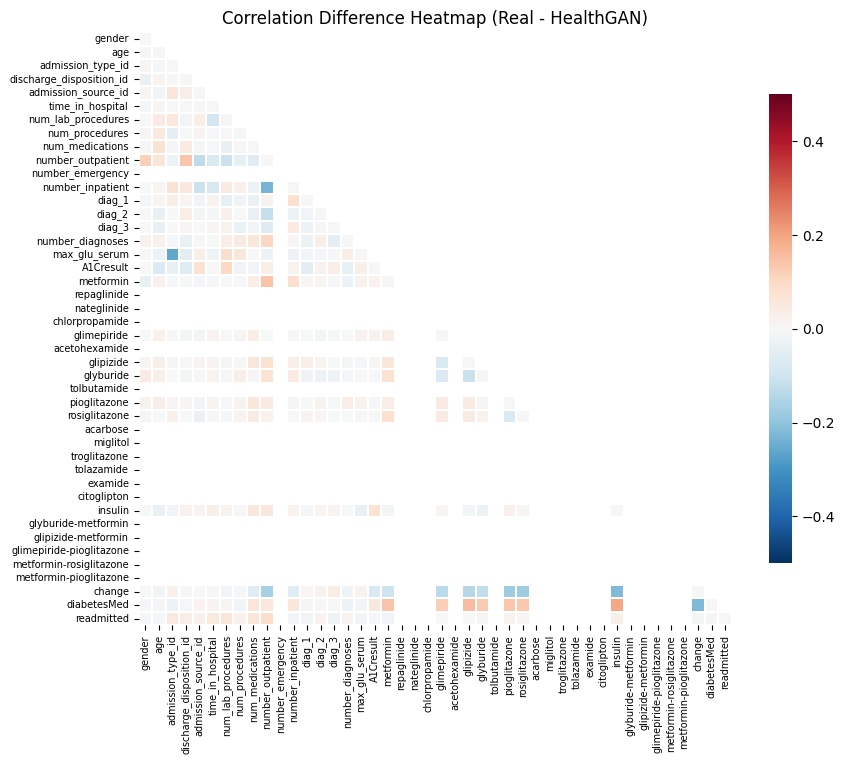
\includegraphics[width=\textwidth]{images/results/corrheat_1}\caption{HealthGAN}\end{subfigure}

\vspace{1ex}
\begin{subfigure}{0.48\textwidth}\centering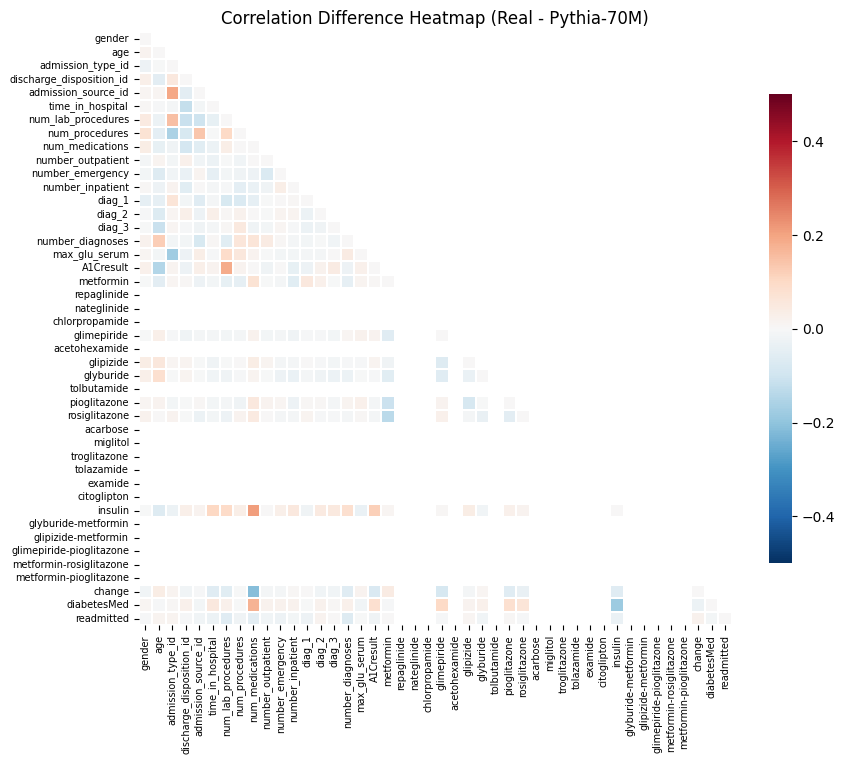
\includegraphics[width=\textwidth]{images/results/corrheat_2}\caption{Pythia-70M}\end{subfigure}\hfill
\begin{subfigure}{0.48\textwidth}\centering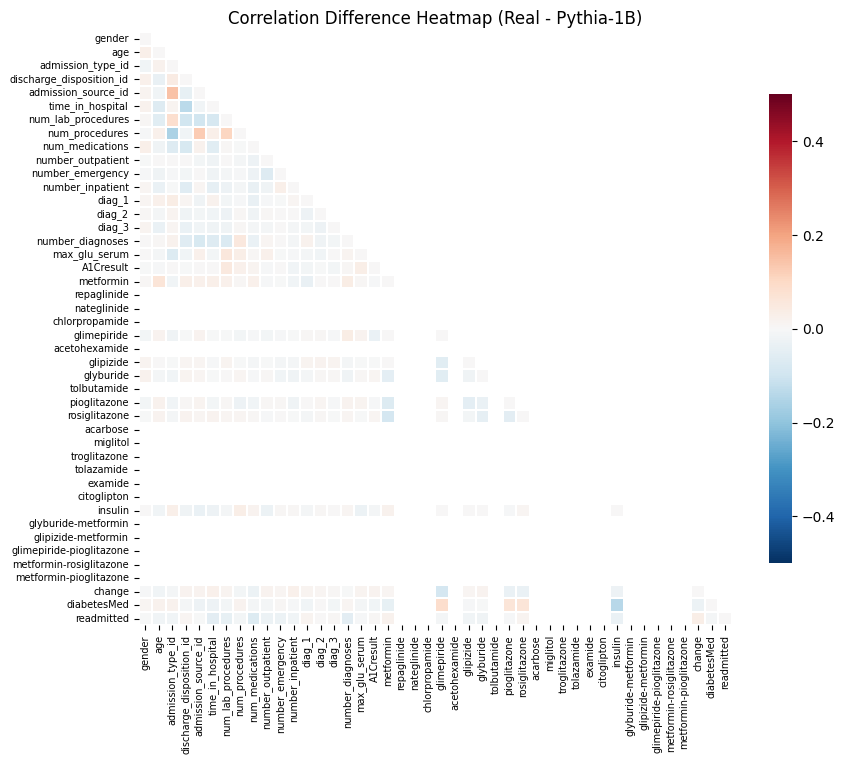
\includegraphics[width=\textwidth]{images/results/corrheat_3}\caption{Pythia-1B}\end{subfigure}

\vspace{1ex}
\begin{subfigure}{0.48\textwidth}\centering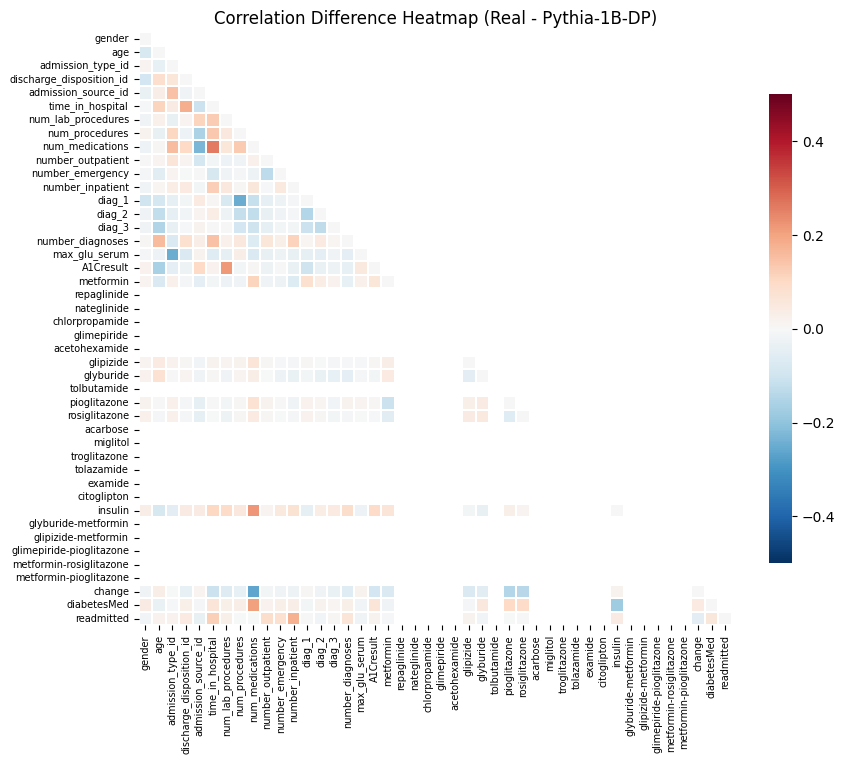
\includegraphics[width=\textwidth]{images/results/corrheat_4}\caption{Pythia-1B-DP}\end{subfigure}
\caption{Correlation-difference heatmaps (real minus synthetic) for all
five generators.}
\label{app:fig:corrheat}
\end{figure}

\section{Cox Proportional-Hazards Estimates}
\label{app:cox}

Figure~\ref{app:fig:cox} gives the Cox hazard-ratio plots (real in black
versus synthetic in colour, with shaded rows marking non-overlapping
confidence intervals) for all five generators, extending the contrast of
Figure~\ref{fig:rq2:cox}. The per-generator confidence-interval overlap
counts are reported in Table~\ref{tab:rq2:cox}.

\begin{figure}[H]
\centering
\begin{subfigure}{0.48\textwidth}\centering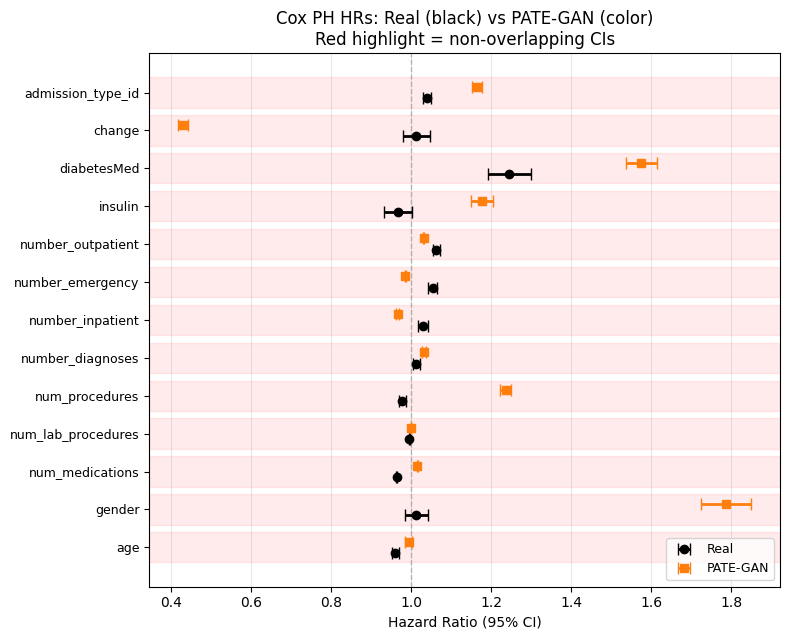
\includegraphics[width=\textwidth]{images/results/cox_0}\caption{PATE-GAN (0/13)}\end{subfigure}\hfill
\begin{subfigure}{0.48\textwidth}\centering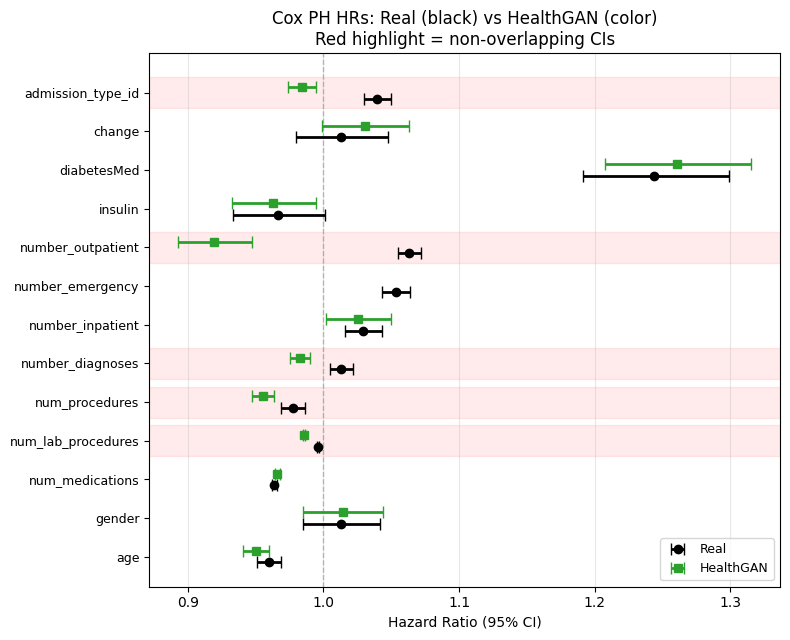
\includegraphics[width=\textwidth]{images/results/cox_1}\caption{HealthGAN (7/12)}\end{subfigure}

\vspace{1ex}
\begin{subfigure}{0.48\textwidth}\centering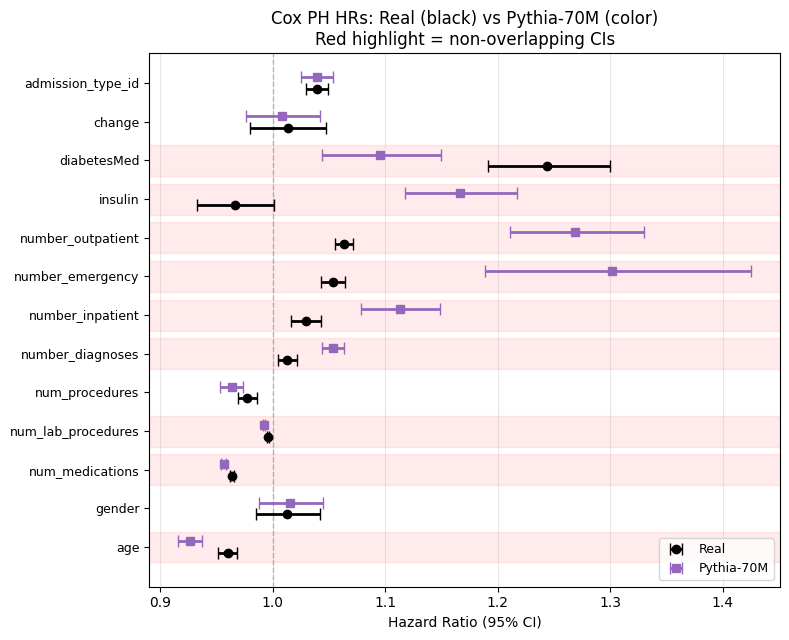
\includegraphics[width=\textwidth]{images/results/cox_2}\caption{Pythia-70M (4/13)}\end{subfigure}\hfill
\begin{subfigure}{0.48\textwidth}\centering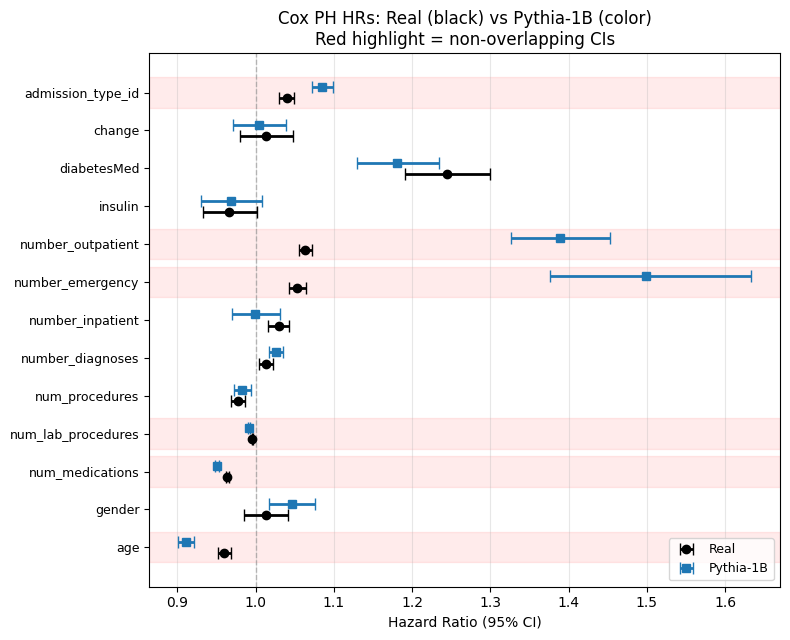
\includegraphics[width=\textwidth]{images/results/cox_3}\caption{Pythia-1B (7/13)}\end{subfigure}

\vspace{1ex}
\begin{subfigure}{0.48\textwidth}\centering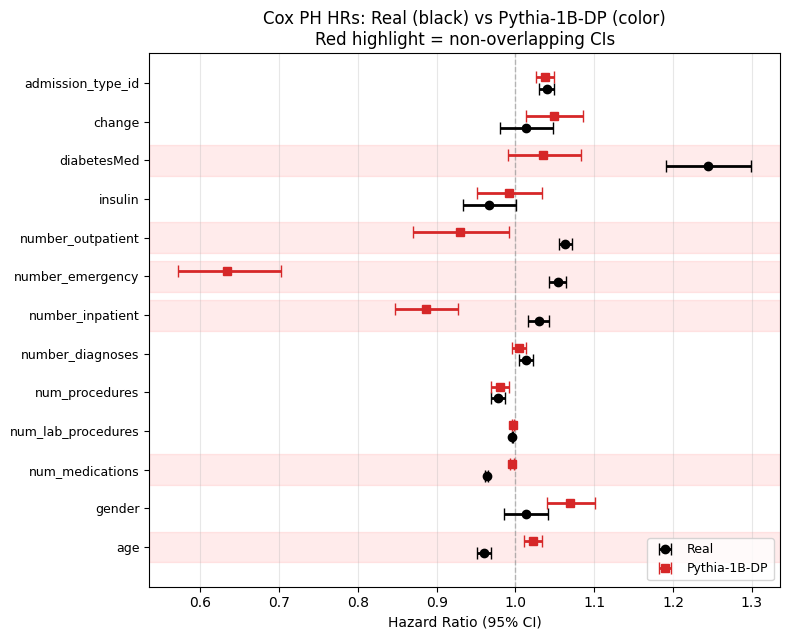
\includegraphics[width=\textwidth]{images/results/cox_4}\caption{Pythia-1B-DP (7/13)}\end{subfigure}
\caption{Cox hazard-ratio estimates with $95\%$ confidence intervals for
all five generators; subcaptions report the overlap count with the real
intervals.}
\label{app:fig:cox}
\end{figure}

% --------------------------------------------------------------

\chapter{Per-Attribute Privacy Risk}
\label{app:privacy-detail}

% TODO: Detailed per-attribute breakdown of attribute-inference advantage
% (§4.2). The main text reports max advantage; here, list every attribute
% × generator cell with the actual value.

% --------------------------------------------------------------

\chapter{Reproducibility}
\label{app:reproducibility}

\section{Repository Layout}
% TODO: tree-style listing of the project showing
%   thesis/, healthgan/, Pategan/, pythia/, and the shared data/ directory.

\section{Run Commands}
% TODO: shell snippets for each pipeline:

% \begin{verbatim}
% # 1. Preprocess
% python -m thesis.feature_engineering ...
%
% # 2. Generate HealthGAN synthetic data
% python healthgan/generators/sdv_converter.py ... encode
% python healthgan/generators/wgan_for_mac.py 5 64
% python healthgan/generators/sdv_converter.py ... decode samples_99999_5_64.npy
%
% # 3. Generate PATE-GAN synthetic data
% python Pategan/generate_pategan_synthetic.py --epsilon 5.0 --splits train test
%
% # 4. Generate Pythia synthetic data (non-DP)
% python pythia/generate_pythia_synthetic.py --splits train test
%
% # 5. Generate Pythia synthetic data (DP)
% python pythia/generate_pythia_synthetic_dp.py --dp \
%        --target-epsilon 5.0 --target-delta 1e-5
%
% # 6. Evaluate
% jupyter execute thesis/data_analysis.ipynb
% \end{verbatim}

\section{Run Metadata Excerpts}
% TODO: include excerpts from
%   thesis/data/pythia/run_metadata.json
%   thesis/data/pythia/run_metadata_dp.json
% showing achieved_epsilon, training duration, hardware.

\section{Computational Environment}
% TODO: Python version, key library versions (torch, opacus, transformers,
% peft, tensorflow, scikit-learn, lifelines), GPU model and memory, OS.
% Wall-clock time per generator.

% --------------------------------------------------------------

\chapter{HealthGAN Variant Comparison}
\label{app:hg-variants}

This appendix provides the visual diagnostics supporting the sample-selection
analysis of Section~\ref{sec:methods:healthgan:variants}, which compares the
three retained HealthGAN draws (indexed $0$, $3$, and $6$) and carries draw
$0$ forward as representative. The headline fidelity figures --- mean
Kolmogorov--Smirnov statistic and mean correlation difference per draw ---
are given in Table~\ref{tab:hg-variants}; the figures below show that the
three draws are visually indistinguishable from one another and from the
real data on every diagnostic, supporting the use of draw $0$ as a representative sample.

The diagnostics in this appendix were generated in the HealthGAN-only
fidelity analysis of \texttt{data\_analysis.ipynb}, using the real training
partition and the three retained decoded HealthGAN draws labelled
HealthGAN-0, HealthGAN-3, and HealthGAN-6 in that analysis.

\section{Per-Column Marginal Distributions}
\label{app:hg-variants:marginals}

\begin{figure}[H]
\centering
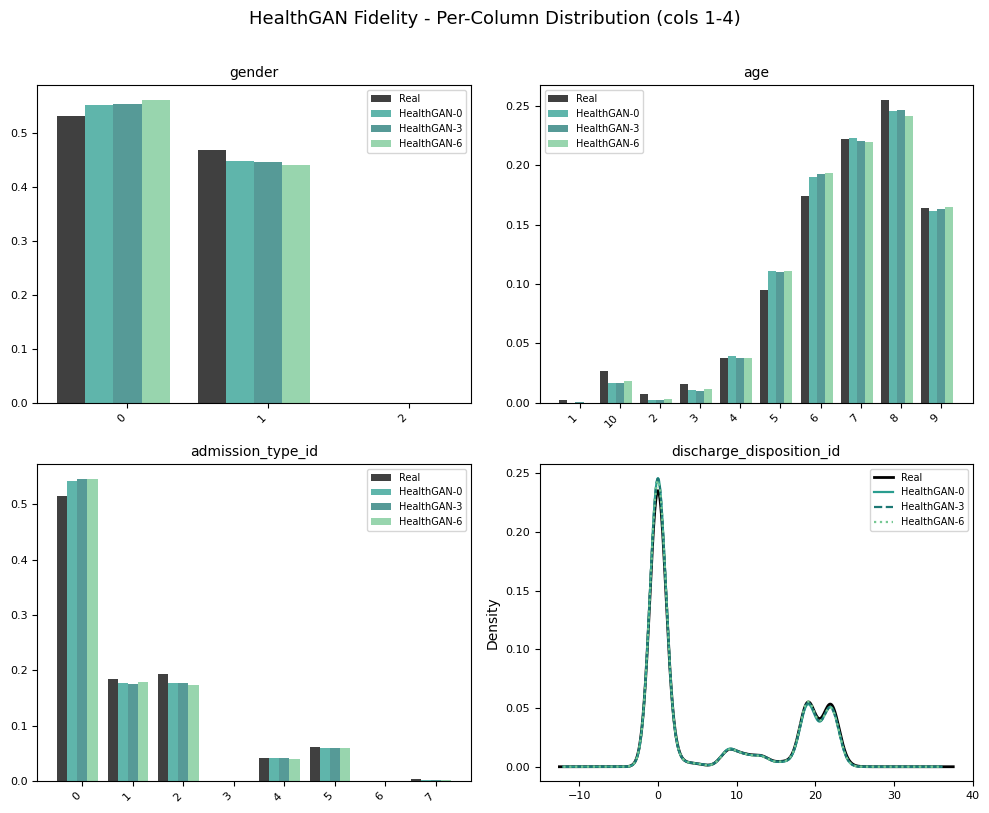
\includegraphics[width=0.92\textwidth]{images/results/hg_marginals_0}
\caption{Per-column marginal distributions, real versus the three HealthGAN
draws (block 1 of 5).}
\label{app:fig:hgmarg0}
\end{figure}

\begin{figure}[H]
\centering
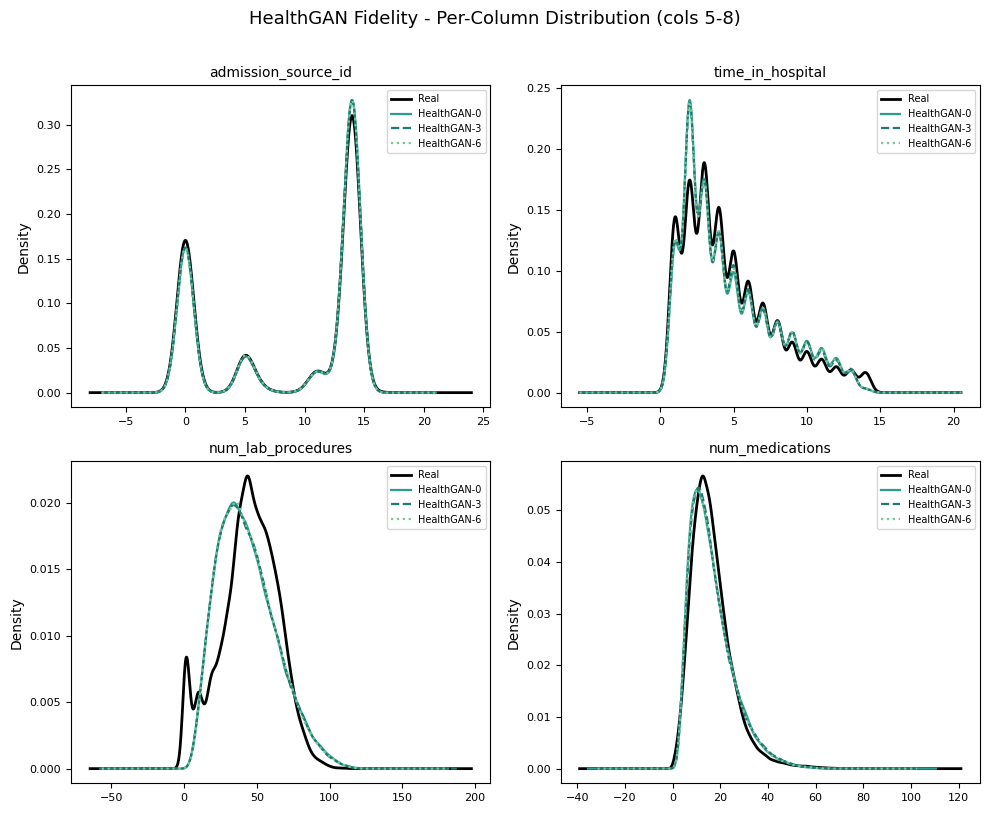
\includegraphics[width=0.92\textwidth]{images/results/hg_marginals_1}
\caption{Per-column marginal distributions, real versus the three HealthGAN
draws (block 2 of 5).}
\label{app:fig:hgmarg1}
\end{figure}

\begin{figure}[H]
\centering
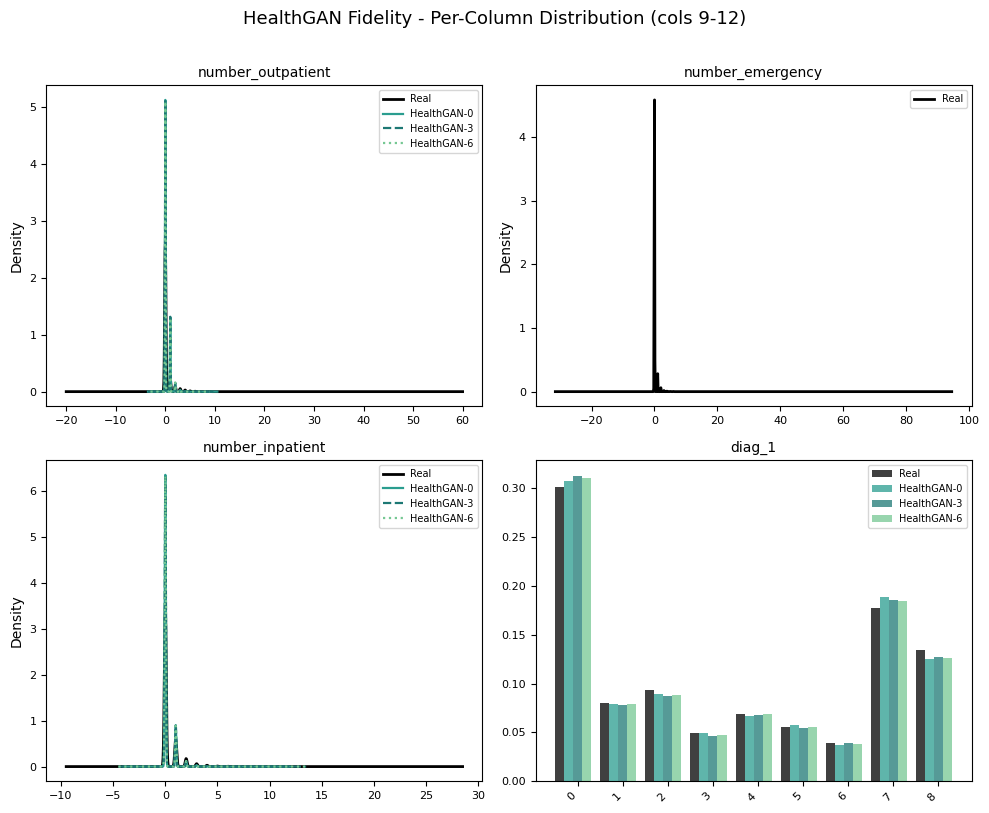
\includegraphics[width=0.92\textwidth]{images/results/hg_marginals_2}
\caption{Per-column marginal distributions, real versus the three HealthGAN
draws (block 3 of 5).}
\label{app:fig:hgmarg2}
\end{figure}

\begin{figure}[H]
\centering
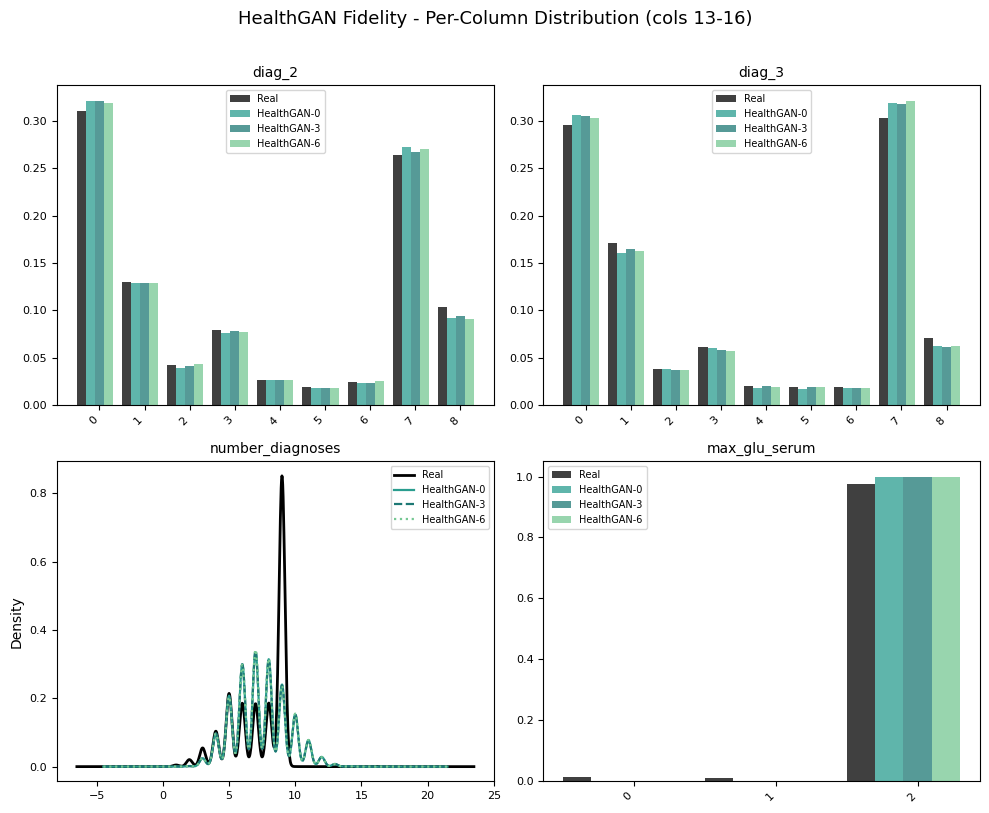
\includegraphics[width=0.92\textwidth]{images/results/hg_marginals_3}
\caption{Per-column marginal distributions, real versus the three HealthGAN
draws (block 4 of 5).}
\label{app:fig:hgmarg3}
\end{figure}

\begin{figure}[H]
\centering
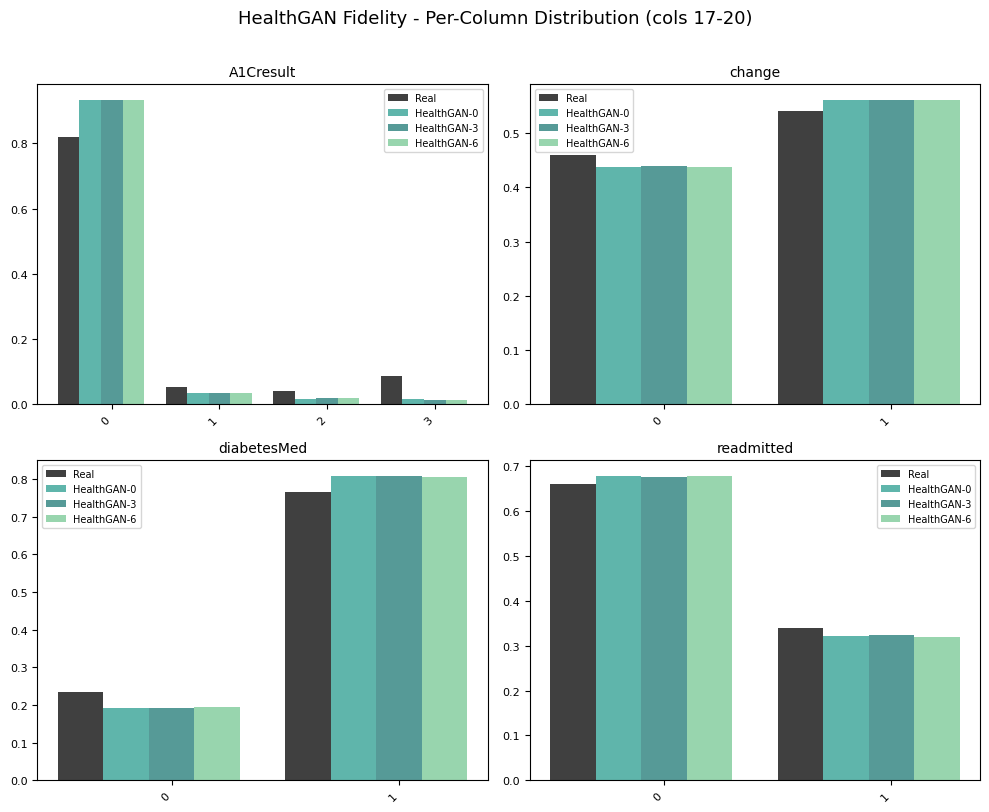
\includegraphics[width=0.92\textwidth]{images/results/hg_marginals_4}
\caption{Per-column marginal distributions, real versus the three HealthGAN
draws (block 5 of 5).}
\label{app:fig:hgmarg4}
\end{figure}

\section{Descriptive Statistics}
\label{app:hg-variants:desc}

\begin{table}[H]
\centering
\small
\caption{Selected per-column means for the real training partition and the
three retained HealthGAN draws.}
\label{app:tab:hg-means}
\begin{tabular}{lrrrr}
\toprule
Column & Real & HG-0 & HG-3 & HG-6 \\
\midrule
gender & 0.468 & 0.448 & 0.446 & 0.440 \\
age & 7.074 & 7.030 & 7.040 & 7.037 \\
admission\_type\_id & 1.082 & 1.011 & 1.004 & 0.999 \\
discharge\_disposition\_id & 6.875 & 6.513 & 6.540 & 6.595 \\
admission\_source\_id & 8.876 & 9.155 & 9.167 & 9.157 \\
time\_in\_hospital & 4.763 & 4.740 & 4.728 & 4.730 \\
num\_lab\_procedures & 44.181 & 43.550 & 43.552 & 43.541 \\
num\_medications & 16.407 & 16.461 & 16.528 & 16.392 \\
number\_outpatient & 0.305 & 0.263 & 0.265 & 0.266 \\
number\_emergency & 0.124 & 0.000 & 0.000 & 0.000 \\
number\_inpatient & 0.320 & 0.174 & 0.173 & 0.173 \\
diag\_1 & 3.523 & 3.504 & 3.494 & 3.487 \\
diag\_2 & 3.480 & 3.420 & 3.413 & 3.418 \\
diag\_3 & 3.415 & 3.417 & 3.408 & 3.440 \\
number\_diagnoses & 7.346 & 7.364 & 7.359 & 7.364 \\
max\_glu\_serum & 1.961 & 2.000 & 2.000 & 2.000 \\
A1Cresult & 0.395 & 0.113 & 0.113 & 0.112 \\
change & 0.540 & 0.562 & 0.561 & 0.562 \\
diabetesMed & 0.766 & 0.809 & 0.808 & 0.805 \\
readmitted & 0.340 & 0.321 & 0.324 & 0.321 \\
\bottomrule
\end{tabular}
\end{table}

\begin{table}[H]
\centering
\small
\caption{Selected per-column standard deviations for the real training
partition and the three retained HealthGAN draws.}
\label{app:tab:hg-std}
\begin{tabular}{lrrrr}
\toprule
Column & Real & HG-0 & HG-3 & HG-6 \\
\midrule
gender & 0.499 & 0.497 & 0.497 & 0.496 \\
age & 1.598 & 1.507 & 1.501 & 1.514 \\
admission\_type\_id & 1.495 & 1.457 & 1.452 & 1.451 \\
discharge\_disposition\_id & 9.186 & 9.033 & 9.044 & 9.066 \\
admission\_source\_id & 6.311 & 6.234 & 6.225 & 6.221 \\
time\_in\_hospital & 3.183 & 3.187 & 3.175 & 3.185 \\
num\_lab\_procedures & 19.964 & 20.144 & 20.051 & 19.963 \\
num\_medications & 8.644 & 9.103 & 9.175 & 9.094 \\
number\_outpatient & 1.127 & 0.539 & 0.539 & 0.541 \\
number\_emergency & 0.650 & 0.000 & 0.000 & 0.000 \\
number\_inpatient & 0.810 & 0.479 & 0.483 & 0.481 \\
diag\_1 & 3.115 & 3.116 & 3.127 & 3.118 \\
diag\_2 & 3.204 & 3.199 & 3.199 & 3.192 \\
diag\_3 & 3.179 & 3.190 & 3.185 & 3.190 \\
number\_diagnoses & 1.972 & 1.996 & 1.996 & 1.992 \\
max\_glu\_serum & 0.255 & 0.010 & 0.004 & 0.010 \\
A1Cresult & 0.916 & 0.472 & 0.470 & 0.470 \\
change & 0.498 & 0.496 & 0.496 & 0.496 \\
diabetesMed & 0.423 & 0.393 & 0.394 & 0.396 \\
readmitted & 0.474 & 0.467 & 0.468 & 0.467 \\
\bottomrule
\end{tabular}
\end{table}

\section{Correlation Structure and Manifold Overlap}
\label{app:hg-variants:corr-pca}

\begin{figure}[H]
\centering
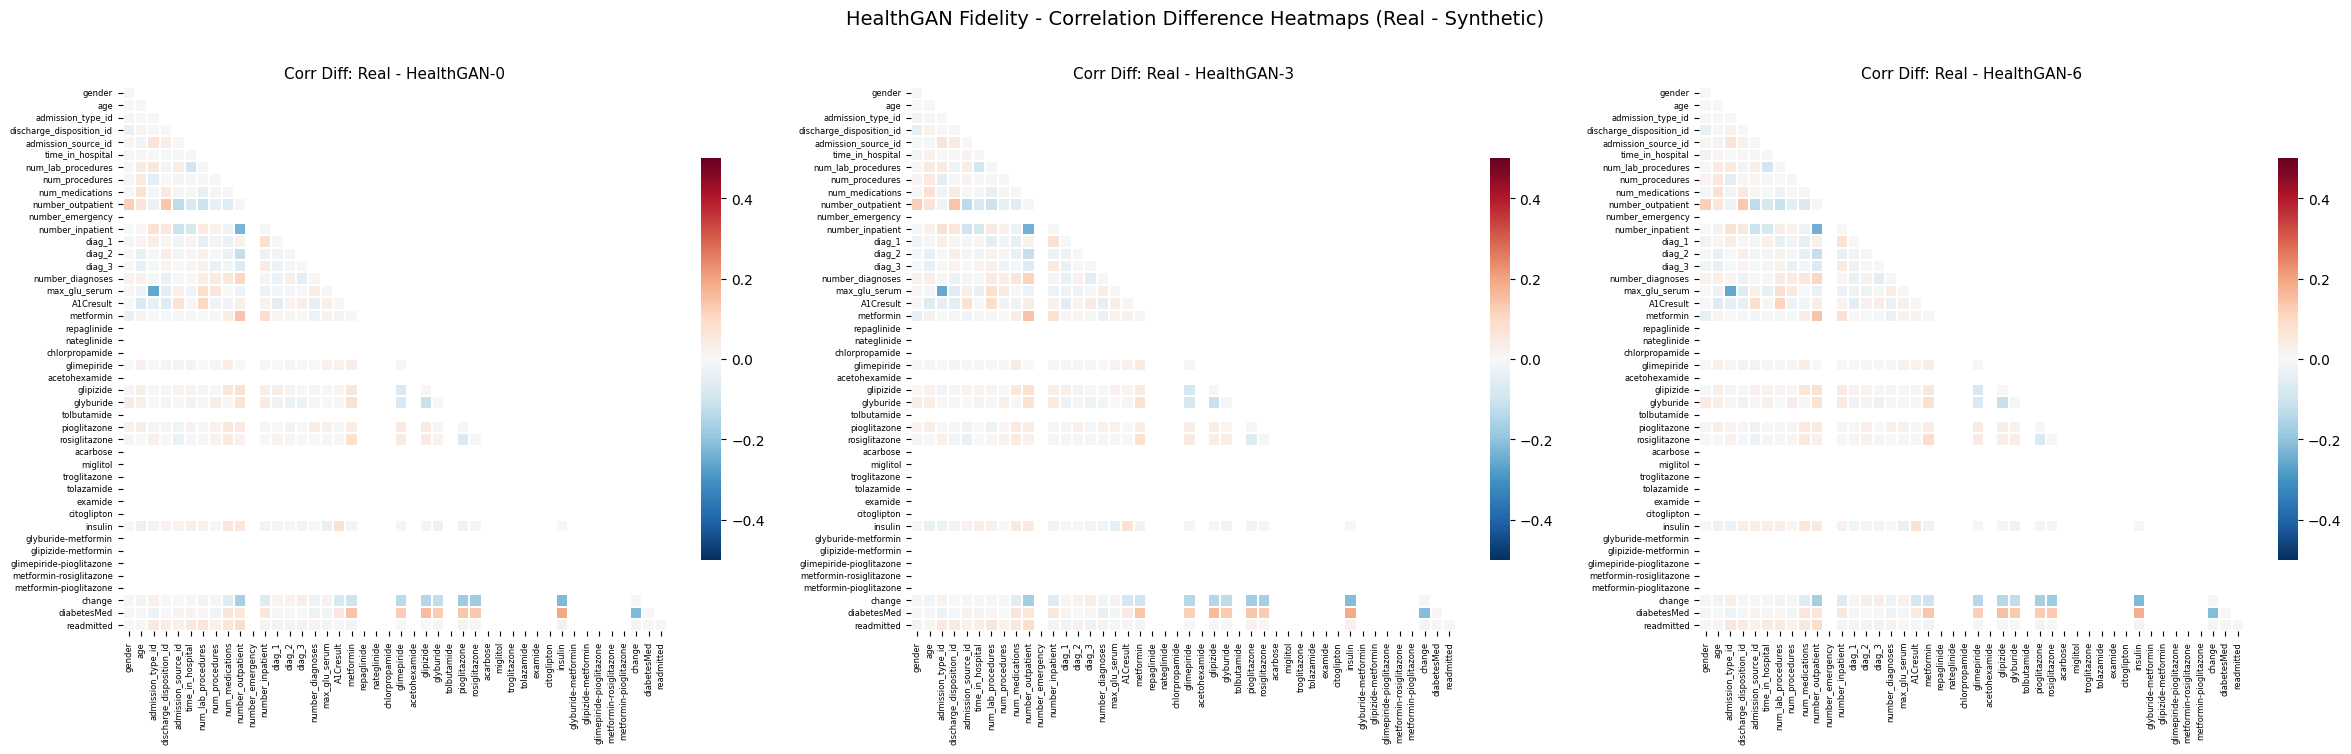
\includegraphics[width=0.92\textwidth]{images/results/hg_corrheat}
\caption{Correlation-difference heatmaps (real minus synthetic) for the
three HealthGAN draws.}
\label{app:fig:hgcorr}
\end{figure}

\begin{figure}[H]
\centering
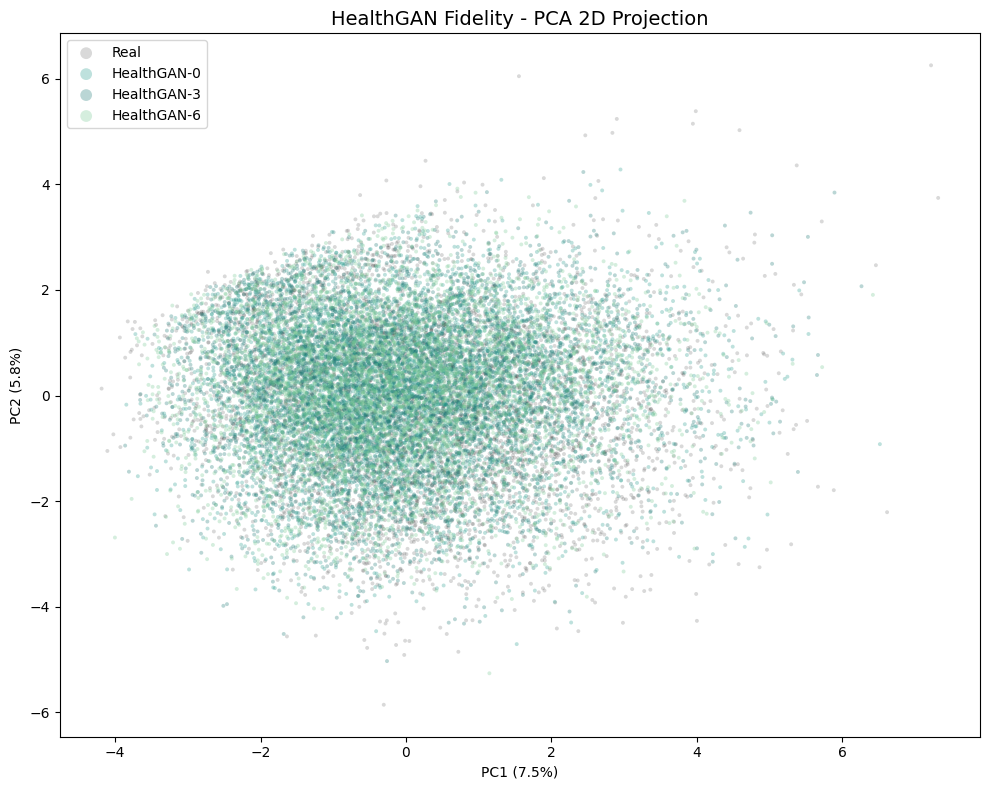
\includegraphics[width=0.7\textwidth]{images/results/hg_pca}
\caption{Two-dimensional PCA projection of the real data and the three
HealthGAN draws; the three draws overlap one another and the real cloud.}
\label{app:fig:hgpca}
\end{figure}
